% Figure: the generator as a superposition of symmetric second differences. Referenced from
% section 6 before prop:scale-evolution. Pure TikZ, schematic (2026-09-18, the author's review:
% illustrate where a schematic carries the point). Three panels: a Cin ray (one displacement
% size), the Matern member (every size, exponential weights), a stable member (every size,
% power-law weights). Line width stands for the weight varpi(dv) of the size; nothing is to scale.

\begin{figure}[t]
\centering
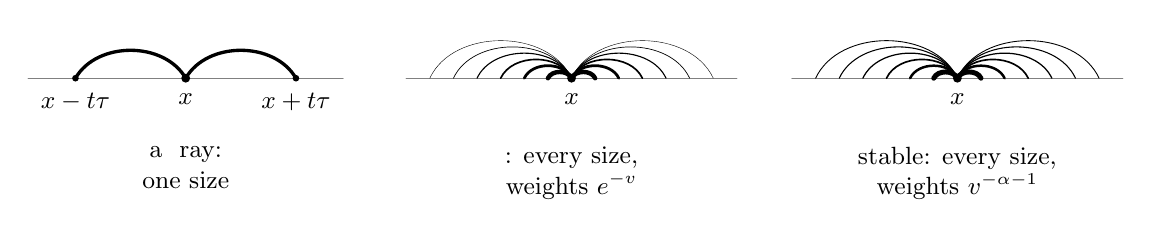
\begin{tikzpicture}[every node/.style={font=\small}, line cap=round, >=stealth]

% --- panel (a): a Cin ray ---------------------------------------------------------------
\begin{scope}[shift={(0,0)}]
\draw[gray] (-2.0,0) -- (2.0,0);
\fill (0,0) circle (1.6pt) node[below=2pt] {$x$};
\draw[line width=1.2pt] (0,0) to[out=60,in=120] (1.4,0);
\draw[line width=1.2pt] (0,0) to[out=120,in=60] (-1.4,0);
\fill (1.4,0) circle (1.2pt) node[below=2pt] {$x + t\tau$};
\fill (-1.4,0) circle (1.2pt) node[below=2pt] {$x - t\tau$};
\node[anchor=north, align=center] at (0,-0.75) {a $\Cin$ ray:\\ one size};
\end{scope}

% --- panel (b): the Matern member ---------------------------------------------------------
\begin{scope}[shift={(4.9,0)}]
\draw[gray] (-2.1,0) -- (2.1,0);
\fill (0,0) circle (1.6pt) node[below=2pt] {$x$};
\foreach \d/\w in {0.3/1.6, 0.6/1.0, 0.9/0.6, 1.2/0.4, 1.5/0.25, 1.8/0.15} {
  \draw[line width=\w pt] (0,0) to[out=65,in=115] (\d,0);
  \draw[line width=\w pt] (0,0) to[out=115,in=65] (-\d,0);
}
\node[anchor=north, align=center] at (0,-0.75) {\Matern{}: every size,\\ weights $e^{-v}$};
\end{scope}

% --- panel (c): a stable member -------------------------------------------------------------
\begin{scope}[shift={(9.8,0)}]
\draw[gray] (-2.1,0) -- (2.1,0);
\fill (0,0) circle (1.6pt) node[below=2pt] {$x$};
\foreach \d/\w in {0.3/1.8, 0.6/0.9, 0.9/0.6, 1.2/0.45, 1.5/0.38, 1.8/0.32} {
  \draw[line width=\w pt] (0,0) to[out=65,in=115] (\d,0);
  \draw[line width=\w pt] (0,0) to[out=115,in=65] (-\d,0);
}
\node[anchor=north, align=center] at (0,-0.75) {stable: every size,\\ weights $v^{-\alpha-1}$};
\end{scope}

\end{tikzpicture}
\caption{The jump part of the generator \ref{eq:evolution-signal}, schematically. At a
position $x$ and a scale $t$ the generator compares $g(x)$ with the average of its two
neighbours at distance $tv$, for every displacement size $v$. It sums the differences with the
weight $\varpi(dv)$, drawn here as line width. A $\Cin$ ray has one size, so its generator is a
single second difference. The \Matern{} member has every size with exponentially decaying
weight, and the sum is a bounded operator, $2\gamma/t$ times the difference between
convolution by the Laplace kernel of range $t$ and the identity. A stable member has every
size with power-law weight, not summable at small sizes, and the sum is the fractional
Laplacian. The Gaussian part of a generator is not drawn: it is the limit of the same
comparison at vanishing size, a multiple of the second derivative.}
\label{fig:generator}
\end{figure}
